%%%%%%%%%%%%%%%%%%%%%%%%%%%%%%%%%%%%%%%%%
% Beamer Presentation
% LaTeX Template
% Version 1.0 (10/11/12)
%
% This template has been downloaded from:
% http://www.LaTeXTemplates.com
%
% License:
% CC BY-NC-SA 3.0 (http://creativecommons.org/licenses/by-nc-sa/3.0/)
%
%%%%%%%%%%%%%%%%%%%%%%%%%%%%%%%%%%%%%%%%%

%----------------------------------------------------------------------------------------
%	PACKAGES AND THEMES
%----------------------------------------------------------------------------------------

%\documentclass{beamer}
\PassOptionsToPackage{dvipsnames}{xcolor}
\documentclass[aspectratio=169]{beamer}
%\documentclass[aspectratio=169]{beamer}
\mode<presentation> {

% The Beamer class comes with a number of default slide themes
% which change the colors and layouts of slides. Below this is a list
% of all the themes, uncomment each in turn to see what they look like.

%\usetheme{default}
%\usetheme{AnnArbor}
%\usetheme{Antibes}
%\usetheme{Bergen}
%\usetheme{Berkeley}
%\usetheme{Berlin}
%\usetheme{Boadilla}
%\usetheme{CambridgeUS}
%\usetheme{Copenhagen}
%\usetheme{Darmstadt}
%\usetheme{Dresden}
%\usetheme{Frankfurt}
%\usetheme{Goettingen}
%\usetheme{Hannover}
%\usetheme{Ilmenau}
%\usetheme{JuanLesPins}
%\usetheme{Luebeck}
%\usetheme{Madrid}
%\usetheme{Malmoe}
%\usetheme{Marburg}
%\usetheme{Montpellier}
%\usetheme{PaloAlto}
%\usetheme{Pittsburgh}
%\usetheme{Rochester}
%\usetheme{Singapore}
%\usetheme{Szeged}
%\usetheme{Warsaw}

% As well as themes, the Beamer class has a number of color themes
% for any slide theme. Uncomment each of these in turn to see how it
% changes the colors of your current slide theme.

%\usecolortheme{albatross}
%\usecolortheme{beaver}
%\usecolortheme{beetle}
%\usecolortheme{crane}
%\usecolortheme{dolphin}
%\usecolortheme{dove}
%\usecolortheme{fly}
%\usecolortheme{lily}
%\usecolortheme{orchid}
%\usecolortheme{rose}
%\usecolortheme{seagull}
%\usecolortheme{seahorse}
%\usecolortheme{whale}
%\usecolortheme{wolverine}

%\setbeamertemplate{footline} % To remove the footer line in all slides uncomment this line
%\setbeamertemplate{footline}[page number] % To replace the footer line in all slides with a simple slide count uncomment this line

%\setbeamertemplate{navigation symbols}{} % To remove the navigation symbols from the bottom of all slides uncomment this line
}

\usepackage{tikz}
\usepackage{pdfrender}

\usetikzlibrary{shapes,arrows}
\usepackage[utf8]{inputenc}
\usepackage{fancyhdr, graphicx} % Allows including images
\usepackage{booktabs} % Allows the use of \toprule, \midrule and \bottomrule in tables
%\usepackage[T1]{fontenc}
\usepackage{helvet}
\renewcommand{\familydefault}{\sfdefault}
\usepackage{tikz}
\graphicspath{{images/}} 
\usepackage{mathtools}
\usepackage{geometry}
%\usepackage{xcolor}
%\usepackage[dvipsnames]{xcolor}
\definecolor{myaqua}{rgb}{0.1, 0.4, 0.5}


\setbeamerfont{author}{size=\large}
\setbeamerfont{institute}{size=\normalsize}
\setbeamerfont{title}{size=\LARGE\bfseries}
\setbeamerfont{subtitle}{size=\Large\normalfont\slshape}
\setbeamerfont{date}{size=\large\itshape}
\setbeamercolor{title}{fg = myaqua}
\setbeamercolor{frametitle}{fg=myaqua}
    \setbeamertemplate{itemize item}{\color{myaqua}$\blacksquare$}
%

\setbeamertemplate{title page}
{


%\newgeometry{left=2cm, right=0cm, bottom=10cm}

%\inserttitlegraphic 
%\vbox{{titlegraphic}}
\begingroup
%    \centering
{\usebeamercolor[fg]{titlegraphic}\vspace*{-0.19cm}\hspace*{-0.99cm}\inserttitlegraphic\par}\vskip1em
    \begin{beamercolorbox}[sep=8pt,left]{title}
      \usebeamerfont{title}\inserttitle\par%
      \ifx\insertsubtitle\@empty%
      \else%
        %\vskip0.25em%
        {\usebeamerfont{subtitle}\usebeamercolor[fg]{subtitle}\insertsubtitle\par}%
      \fi%
    \end{beamercolorbox}%
    \vskip1em\par
    \begin{beamercolorbox}[sep=8pt,left]{author}
      \usebeamerfont{author}\insertauthor
    \end{beamercolorbox}
    \begin{beamercolorbox}[sep=5pt,left]{institute}
      \usebeamerfont{institute}\insertinstitute
    \end{beamercolorbox}
    \begin{beamercolorbox}[sep=8pt,left]{date}
      \usebeamerfont{date}\insertdate
    \end{beamercolorbox}
  \endgroup
  \vfill
}



%----------------------------------------------------------------------------------------
%	TITLE PAGE
%----------------------------------------------------------------------------------------


\titlegraphic{\includegraphics[width=15.2 cm]{Back_ground.eps}}


\title{SPE-195036-MS \\ Beyond Steel Casing: Detecting Zonal Isolation in the Borehole Environment} % The short title appears at the bottom of every slide, the full title is only on the title page

\author{Timofey Eltsov, Tadeusz W. Patzek} % Your name
\institute[] % Your institution as it will appear on the bottom of every slide, may be shorthand to save space
{
ANPERC, King Abdullah University of Science and Technology \\ % Your institution for the title page
%\medskip
%\textit{timofey.eltsov@kaust.edu.sa} % Your email address
}
\date{Thursday, 21 March 2019} % Date, can be changed to a custom date

\begin{document}


\begin{frame}
\titlepage % Print the title page as the first slide
\end{frame}


%\begin{frame}
%
%\vspace*{-1.325cm}\hspace*{-0.99cm}\includegraphics[scale=0.0544]{Back_ground.eps}
%
%\LARGE \textcolor{myaqua}{\textbf{SPE-195036-MS}} \\
%\vspace*{0.3cm}
%\textcolor{myaqua}{\textbf{Beyond Steel Casing: Detecting Zonal Isolation in the Borehole Environment}} \\
%\vspace*{0.6cm}
%\large Timofey Eltsov and Tadeusz W. Patzek \\
%\vspace*{0.15cm}
%King Abdullah University of Science and Technology
%
%\end{frame}


\setbeamertemplate{footline}[text line]{%
  \parbox{\linewidth}{\vspace*{-0.7cm}\hspace*{-1cm}
\includegraphics[scale=0.0544]{inner_slides.eps}}}

%\setbeamertemplate{headline}[frame number]%

\setbeamertemplate{frametitle}{\nointerlineskip  
    \begin{beamercolorbox}[wd=\paperwidth,ht=2.75ex,dp=1.375ex]{frametitle}
        \hspace*{2ex}\insertframetitle \hfill {\tiny\insertframenumber} \hspace*{1ex}%
    \end{beamercolorbox}}


%----------------------------------------------------------------------------------------
%	PRESENTATION SLIDES
%----------------------------------------------------------------------------------------

%------------------------------------------------
%\section{First Section} % Sections can be created in order to organize your presentation into discrete blocks, all sections and subsections are automatically printed in the table of contents as an overview of the talk
%------------------------------------------------

%
%\begin{frame}{Motivation}
%
%\begin{block}{}
%    \textbf{The objective} is to verify cement quality (integrity and solidification state) in a borehole environment 
%%behind the non-conductive casing using cement with iron powder and induction logging tool
%\end{block}
%  
%\begin{block}{}
%    \textbf{The focus}  is on numerical simulation of cement containing iron powder magnetization and measurements of magnetic response
%\end{block}
%
%\begin{block}{}
%    \textbf{The solution} is to compute tool parameters - distance between coils, operating frequencies, coil parameters etc.  
%\end{block}
%
%
%\end{frame}


%
%
%%
%\begin{frame}{Objective of the project}
%
%\begin{block}{}
%    \textbf{The objective} is to verify cement quality (integrity and solidification state) in a borehole environment 
%%behind the non-conductive casing using cement with iron powder and induction logging tool
%\end{block}
%  
%\begin{block}{}
%    \textbf{The focus}  is on numerical simulation of cement containing iron powder magnetization and measurements of magnetic response
%\end{block}
%
%\begin{block}{}
%    \textbf{The solution} is to compute tool parameters - distance between coils, operating frequencies, coil parameters etc.  
%\end{block}
%
%
%\end{frame}
%
%----------------------------------------------------------
%
%\begin{frame}
%\frametitle{Application}
%
%\begin{columns}[c] 
%\column{.6\textwidth} % Right column and width
%%{\footnotesize
%
%
%\begin{small}
%\begin{itemize}
%
%\item The main cost of geothermal energy production is electrical power consumption of the submersible pumps
%\item Pumps are forced to overcome losses in closed environment 
%\item Corrosion and mineral precipitation is often observed in geothermal wells 
%\item Bad cement job can result in well bore breakdown and power plant shutdown
%\end{itemize}
%\end{small}
%
%\column{.4\textwidth} % Left column and width
%
%\begin{center}
%\includegraphics[scale=0.11]{Krafla_geothermal.eps}
%\end{center}
%
%\begin{center}
%\tiny{Krafla geothermal station, Iceland - 60 MW}
%\end{center}
%
%\end{columns}
%
%\end{frame}

%
%----------------------------------------------------------
%

\begin{frame}
\frametitle{Motivation}
\begin{columns}[c]
\column{.4\textwidth} % Right column and width
%{\footnotesize



\begin{center}

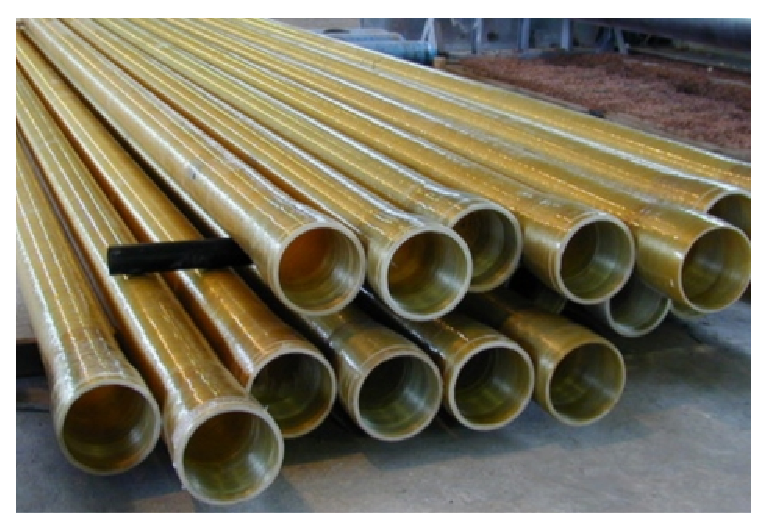
\includegraphics[scale=0.34]{pipe2.eps}

\tiny{Fiberglass composite pipes (zst.ru)}

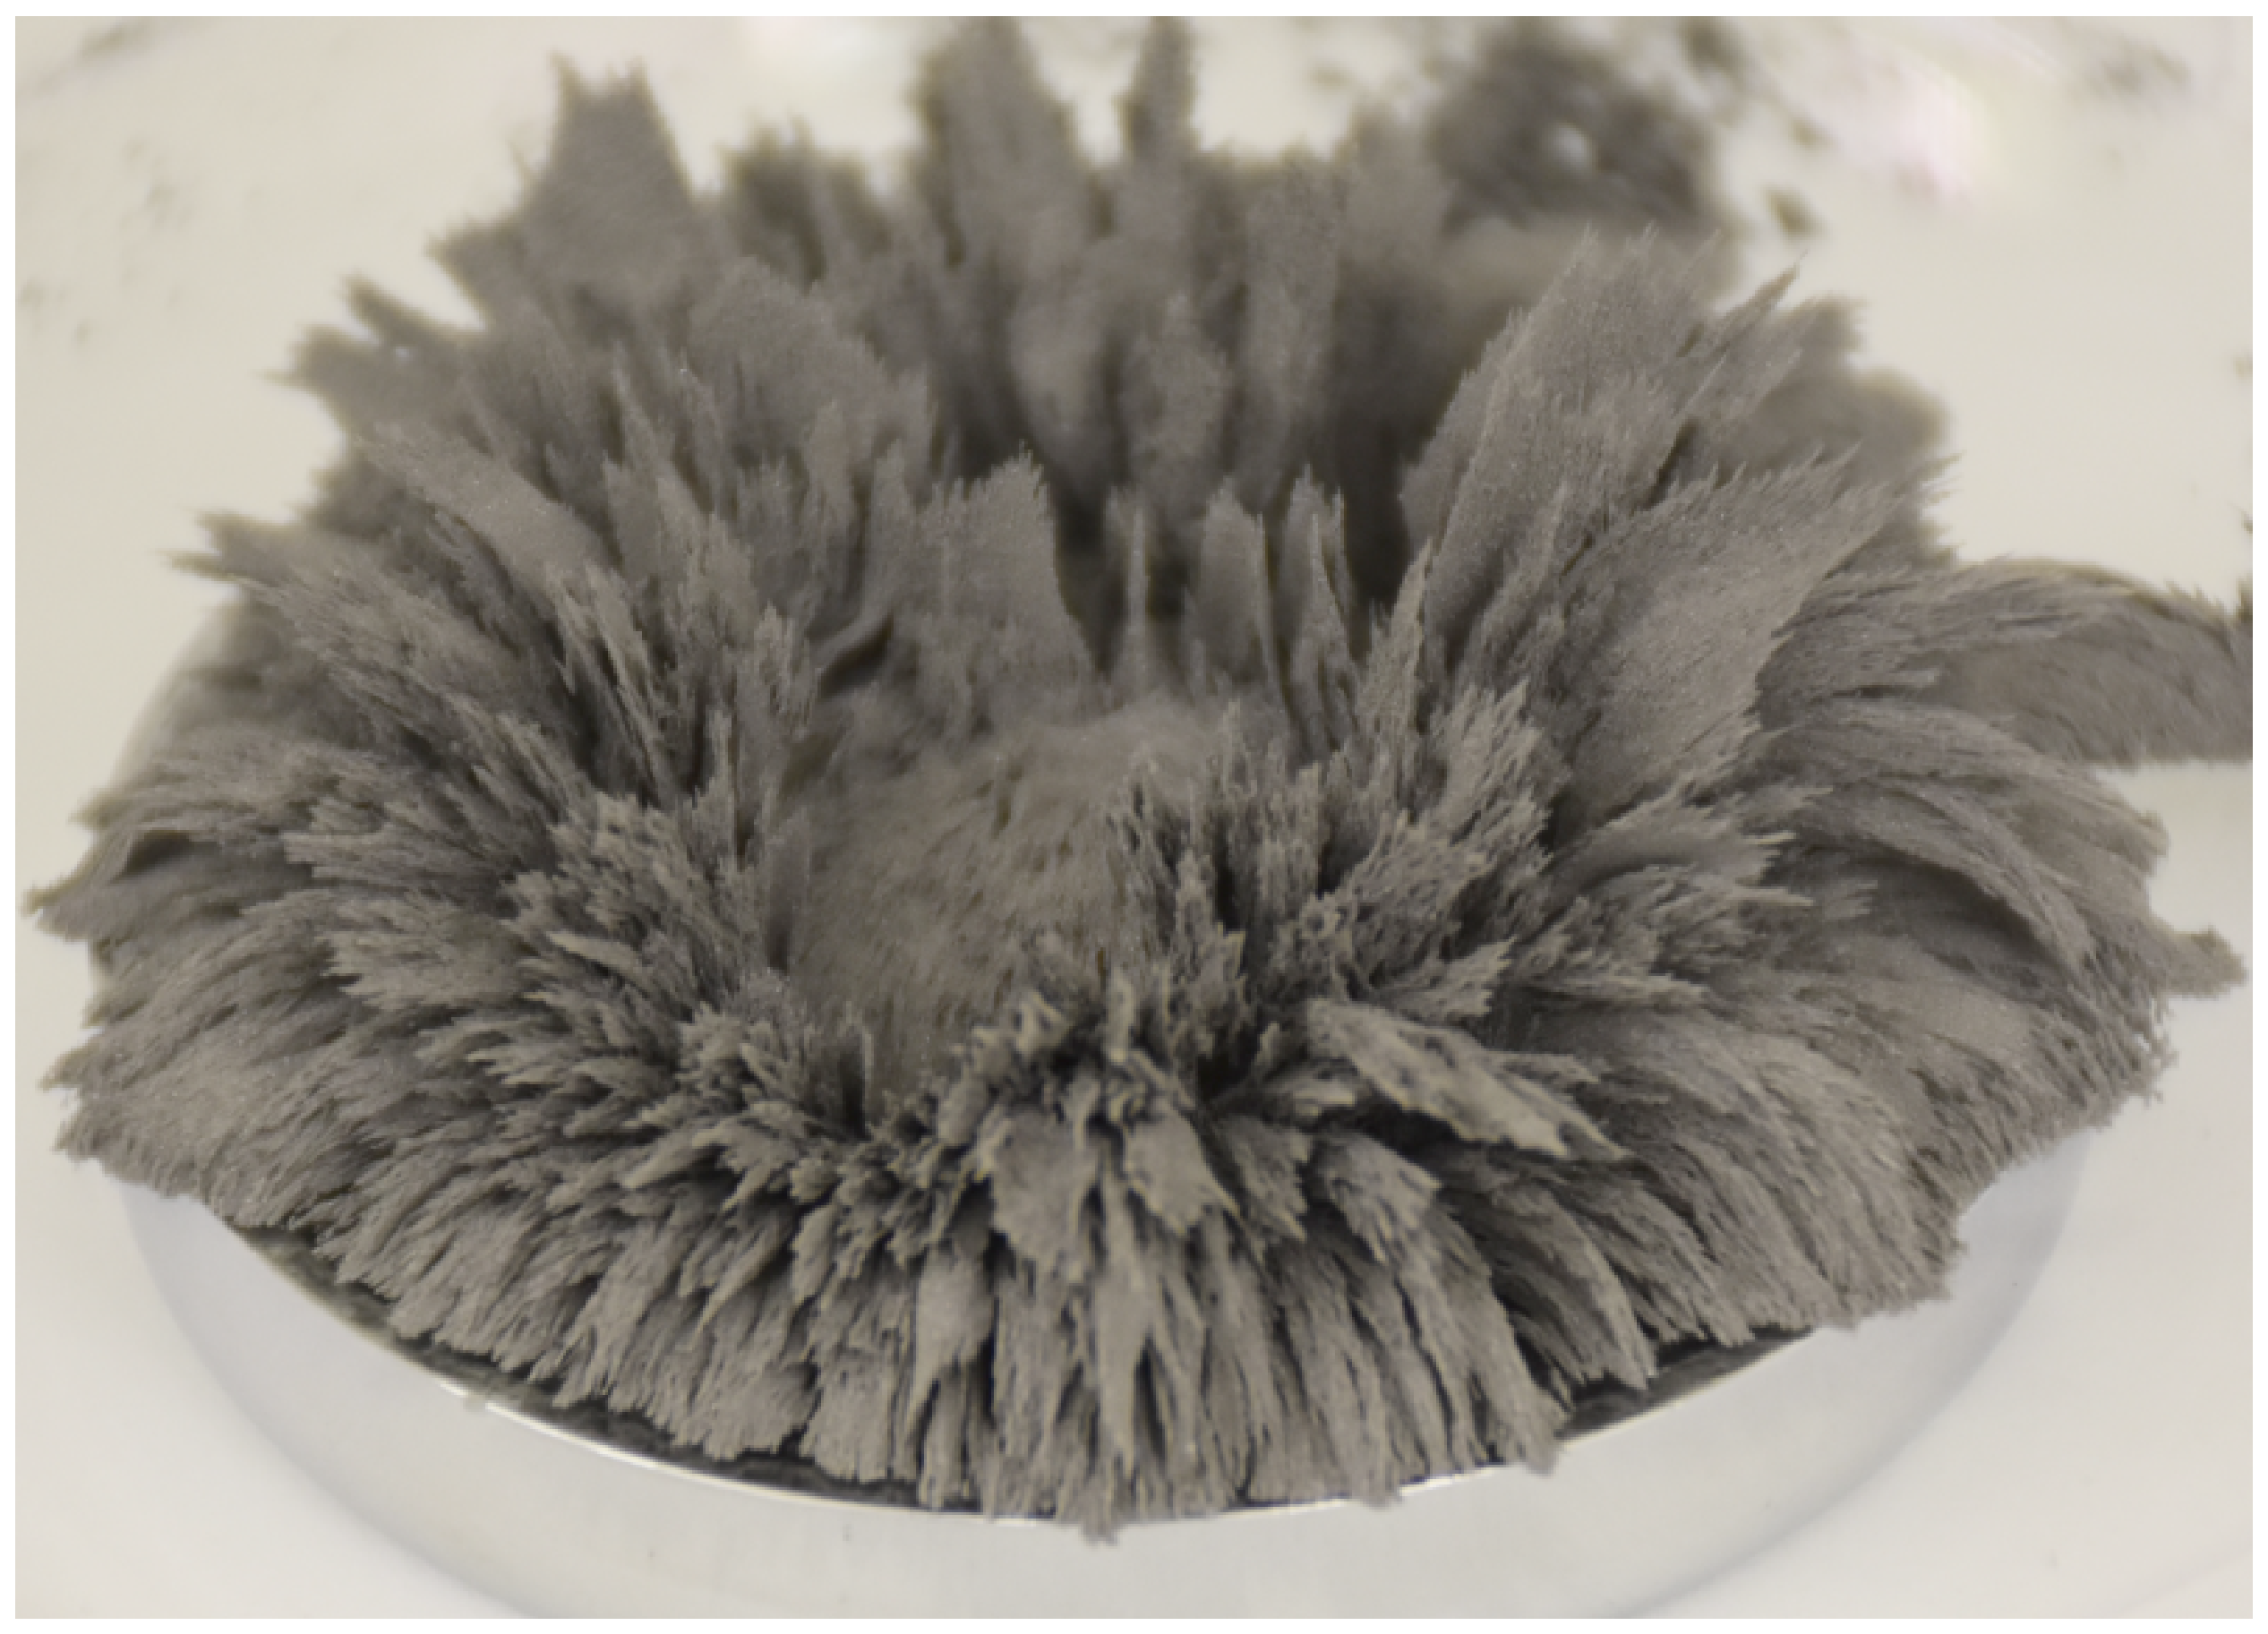
\includegraphics[scale=0.1]{iron_powder.eps}

\end{center}

\vspace{1.9cm}

\column{.65\textwidth} % Left column and width

\begin{small}
\begin{itemize}

\item Electrically resistive composite casing materials are being introduced to the oil and gas industry
\item Composite tubulars are 4 times lighter than made of steel, withstand same pressure and load, resistant to corrosion and lasts more than twice longer
\item The use of EM transparent casing materials requires the development of appropriate geophysical methods
\item Presence of conductive particles in the cement allows to increase its displacement and check its quality using EM 
\item We use magnetic sensors to verify quality of the cement behind casing

\end{itemize}
\end{small}

\vspace{2.5cm}

\end{columns}

\end{frame}
%
%
%%---------------------------------------------------------------------------------------
%%%
%%\subsection{Subsection Example} % A subsection can be created just before a set of slides with a common theme to further break down your presentation into chunks
%%
\begin{frame}{Magnetic susceptibility logging, borehole environment}

\begin{columns}[c] 

\column{.7\textwidth} % Right column and width
\begin{block}{}
\begin{itemize}
	\item Borehole environment is magnetized  by \textcolor{blue} {a low frequency} induction tool
	\item Measurements can be made by coils or sensors (Flux gate magnetometers)
	\item Alternating magnetic field provides necessary  \textcolor{blue} {noise immunity} of logging measurements and excludes the influence of the geomagnetic field
\end{itemize}

\end{block}


\column{.1\textwidth} % Left column and width
\includegraphics[scale=0.14]{tool_view.eps}
\end{columns}


\end{frame}
%
%------------------------------------------------
%

\begin{frame}
\frametitle{Magnetic susceptibility logging}
\begin{itemize}
\item Transmitter coil generates magnetic field, that produces eddy current in the formation 
\item The secondary magnetic field is registered by receiver coil
\item Only vertical component of magnetic field is considered - $H_z$
\end{itemize}
\begin{center}
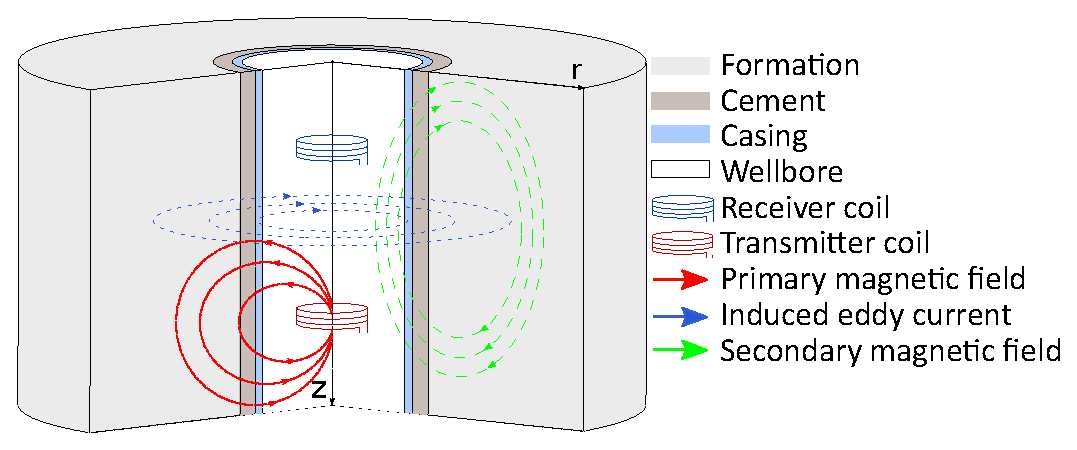
\includegraphics[scale=0.62]{Borehole_big.eps}
\end{center}
\end{frame}
%
%------------------------------------------------
%
\begin{frame}
\frametitle{Magnetic susceptibility logging}
\begin{itemize}
\item Primary and secondary magnetic fields induce an electromotive force in the receiver coil
\item Primary magnetic field is much stronger than secondary one
\item Magnetic susceptibility tool is calibrated by response measurement in the air and its exclusion from the measured signal 
\item There is no secondary magnetic field in the air
\end{itemize}
\end{frame}
%
%------------------------------------------------
%
\begin{frame}
\frametitle{Tool response measurement}


\begin{columns}[c] % The "c" option specifies centered vertical alignment while the "t" option is used for top vertical alignment

\column{.4\textwidth} % Right column and width
{
\begin{equation}
H_{z,m} =\textcolor{red}{H_{z,p}} + \textcolor{green}{H_{z,s}}
\end{equation}
}

\begin{equation}
\textcolor{green}{H_{z,s}} = H_{z,m} - \textcolor{red}{H_{z,p}}
\end{equation}

\vspace{\baselineskip}
$H_{z,m}$ - measured magnetic field, \textcolor{red}{$H_{z,p}$} - primary magnetic field, \textcolor{green}{$H_{z,s}$} - secondary magnetic field


\column{.4\textwidth} % Left column and width

\includegraphics[scale=0.8]{coils.eps}
\end{columns}

\end{frame}
%
%------------------------------------------------
%
\begin{frame}
\frametitle{Formulation of the problem}

\begin{columns}[c] 
\column{.63\textwidth} % Right column and width
%{\footnotesize

\footnotesize
\begin{enumerate} 
\item All layers are isotropic and homogeneous
\item Media consists of cylindrical layers with constant electrical parameters in the direction parallel to Z axis
\item Wellbore is an infinite column of liquid, its axis coincides with the axes of all layers
\item Coils axes coincides with the axis of the wellbore
\item Compared with the size of the tool coils are considered to be point dipoles
\end{enumerate} 

\hspace*{1 cm} \textbf{Geoelectric table}
\begin{tiny}
\begin{table}
\begin{tabular}{c|c|c|c|c}

{Parameter} & {Wellbore} & {Casing}& {Cement} & {Formation} \\
\midrule
Radius, $m$             & 0.07 & 0.10 & 0.15 &  \\
Resistivity, $\Omega\cdot m$    & 2 & $10^8$ & 1 - 1000 & 50 \\
Magnetic permeability & 1 & 1 & 1, 1.25, 1.5, 2 & 1  \\
%Relative permittivity & 1 & 1 & 1 & 1 \\

\end{tabular}
\end{table}
\end{tiny}

\column{.38\textwidth} % Left column and width
\begin{center}
	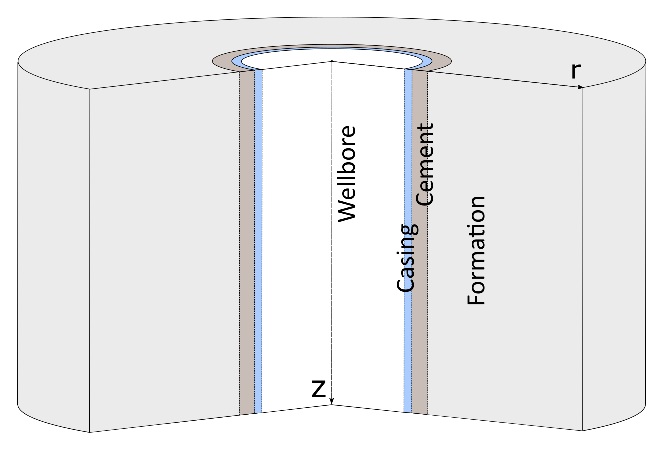
\includegraphics[scale=0.5]{Borehole_big_2.eps}


\end{center}
\end{columns}

\end{frame}
%
%------------------------------------------------
%
%\begin{frame}
%\frametitle{Tool response modeling}
%
%Helmholtz equation in cylindrical coordinates ($\rho$, $\varphi$, $z$):
%\begin{equation}
%\frac{1}{\rho} \frac{\partial}{\partial \rho} \Big( \rho \frac{\partial A_z}{\partial \rho} \Big) + \frac{1}{\rho^2}  \frac{\partial^2 A_z}{\partial^2 \varphi} + \frac{\partial^2 A_z}{\partial^2 z} + k^2 A_z = 0
%\end{equation}
%
%\begin{equation}
%H_z = k^2 A_z + \frac{\partial^2 A_z}{\partial^2 z}; \;  H_\rho = \frac{\partial^2 A_z}{\partial \rho\partial z}; \; E_\varphi = i \omega \mu \frac{\partial A_z}{\partial \rho}.
%\end{equation}
%
%
%Wave number:
%\begin{equation}
%k^2 =  - i \omega \mu \sigma
%\end{equation}
%
%
%\vspace{\baselineskip}
%$A_z$ - vector potential, $\omega$ - circular frequency, $\mu = \mu_r \mu_0$ - magnetic permeability ($\mu_r$ - relative, $\mu_0$ - permeability of vacuum), $\sigma = 1/\Omega$ - conductivity, $\Omega$ - resistivity
%
%\end{frame}
%
%%------------------------------------------------
%
%\begin{frame}
%\frametitle{Boundary conditions, vector potential}
%\begin{small}
%At the interfaces, tangential components of the electric and magnetic field are continuous functions:
%
%\begin{equation}
%\mu_m \frac{\partial A_{z, m}}{\partial \rho} = \mu_{m+1} \frac{\partial A_{z, m+1}}{\partial \rho}
%\end{equation}
%
%\begin{equation}
%k_m^2 A_{z,m} + \frac{\partial^2 A_{z,m}}{\partial^2 z} = k_{m+1}^2 A_{z,m+1} + \frac{\partial^2 A_{z,m+1}}{\partial^2 z}
%\end{equation}
%
%Near the origin of coordinates system the function $A_z$ tends to:
%\begin{equation}
%A_z^{0} = \frac{M e^{-ik_1 R}}{4 \pi R}, \; R = \sqrt{r^2+z^2}  \to	0
%\end{equation}
%
%$M$ - magnetic moment of the coil, $m$ -number of the layer ($m = 1$ - wellbore, $m = 2$ - casing, etc.)
%\end{small}
%\end{frame}
%
%%------------------------------------------------
%
%\begin{frame}
%\frametitle{Vector potential in the first layer}
%
%Vector potential in the wellbore is:
%
%\begin{equation}
%A_{z, 1} = \frac{M}{4\pi} \left( \frac{ e^{-ik_1 R}}{R} + \frac{2}{\pi} {\int_0^\infty C_1 I_0 (\lambda_1 r) \cos \lambda z \; d \lambda}\right)
%\end{equation}
%
%\begin{equation}
%\lambda_m = \sqrt{\lambda^2 + i \sigma \mu  \omega }\: , \: R>0
%\end{equation}
%
%$M$ - magnetic moment of the coil, $\lambda$ is the variable of separation, $r$ - radial distance, $z$ - distance between coils,  $\omega$ - circular frequency, $\mu$  - magnetic permeability, $\sigma$ - conductivity, $C_1$ - constant obtained from boundary conditions, carries information about borehole environment
%
%\end{frame}

%------------------------------------------------
%
%\begin{frame}
%\frametitle{Geoelectric model}
%\begin{center}
%	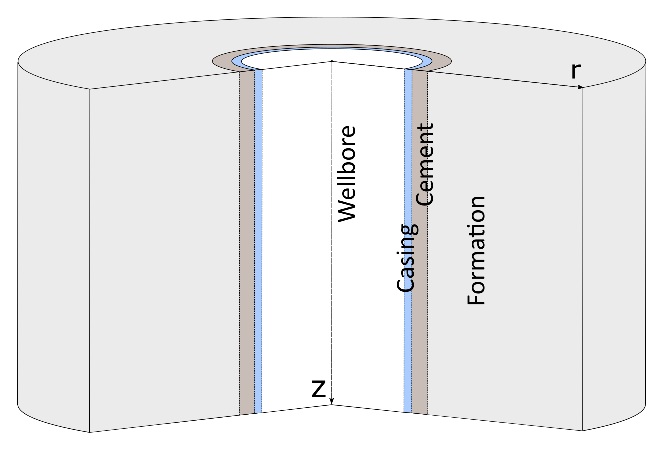
\includegraphics[scale=0.35]{Borehole_big_2.eps}
%\end{center}
%\begin{table}
%\begin{tabular}{|c|c|c|c|c|}
%\toprule
%\textbf{Parameter} & \textbf{Wellbore} & \textbf{Casing}& \textbf{Cement} & \textbf{Formation} \\
%\midrule
%Radius, $m$             & 0.07 & 0.10 & 0.15 &  \\
%Resistivity, $\Omega\cdot m$    & 2 & $10^8$ & 100 & 50 \\
%Magnetic permeability & 1 & 1 & 1 & 1  \\
%Relative permittivity & 1 & 1 & 1 & 1 \\
%\bottomrule
%\end{tabular}
%
%\end{table}
%\end{frame}
%
%------------------------------------------------
%
%\begin{frame}
%\frametitle{Numerical calculation}
%
%Modeling of response has been performed in order to study:
%
%\begin{itemize}
%\item Drilling fluid \textcolor{blue} {resistivity}
%\item Formation \textcolor{blue} {resistivity}
%\item Cement \textcolor{blue} {hardening}
%\item Magnetic \textcolor{blue} {permeability} of the cement (\textcolor{blue} {amount} of magnetic particles)
%\end{itemize}
%
%\begin{columns}[c] 
%\column{.4\textwidth} % Right column and width
%{\footnotesize
%
%Secondary magnetic field (\textcolor{green}{$H_{z,s}$}) will be shown on upcoming slides as it carries information about formation under study.
%}
%
%\column{.4\textwidth} % Left column and width
%
%\includegraphics[scale=0.6]{coils.eps}
%
%\end{columns}
%
%\end{frame}
%
%%------------------------------------------------
%\begin{frame}
%
%\frametitle{Real part of secondary magnetic field, $H_{z,s}$}
%\begin{itemize}
%\item \textcolor{green}{$H_{z,s}$} \textcolor{blue} {is not} influenced by resistivity of mud, formation and cement
%\item Amount of magnetic powder in the cement has strong influence on 
%\textcolor{green} {{$H_{z,s}$}} i.e. useful information about cementing \textcolor{blue} {quality} can be extracted from it! 
%\end{itemize}
%
%Curves for different resistivity of cement, mud and formation overlap. 
%Here is typical pattern of \textcolor{green}{$H_{z,s}$} vs. tool length ($\mu_{cement} = 1.5$):
%\begin{center}
%
%\includegraphics[scale=0.5]{Cem_re.eps}
%\end{center}
%\end{frame}
\begin{frame}

\frametitle{Amount of magnetic powder in the cement, frequency = 1 kHz}


\begin{minipage}{0.49\linewidth}
\center{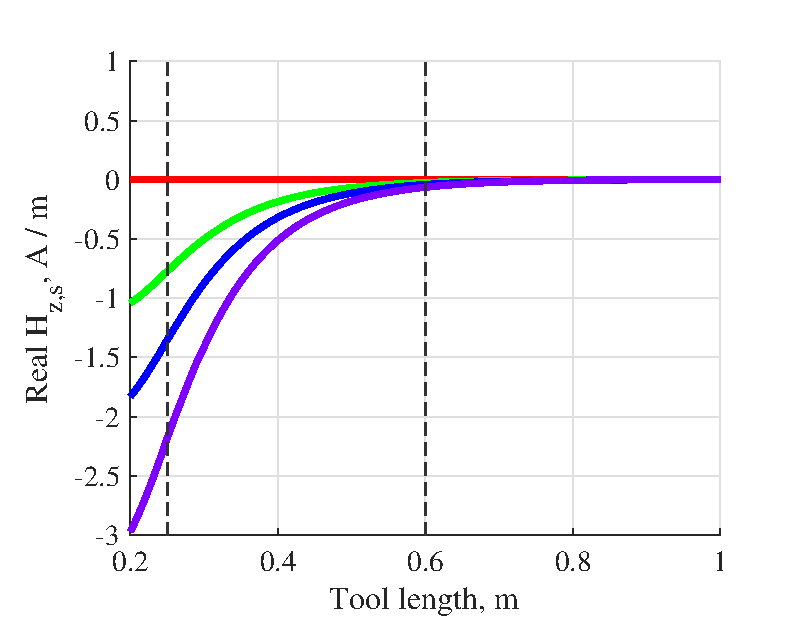
\includegraphics[clip,scale=0.44]{H_re_mu.eps} \\ }
\end{minipage}
\hfill
\begin{minipage}{0.49\linewidth}
\center{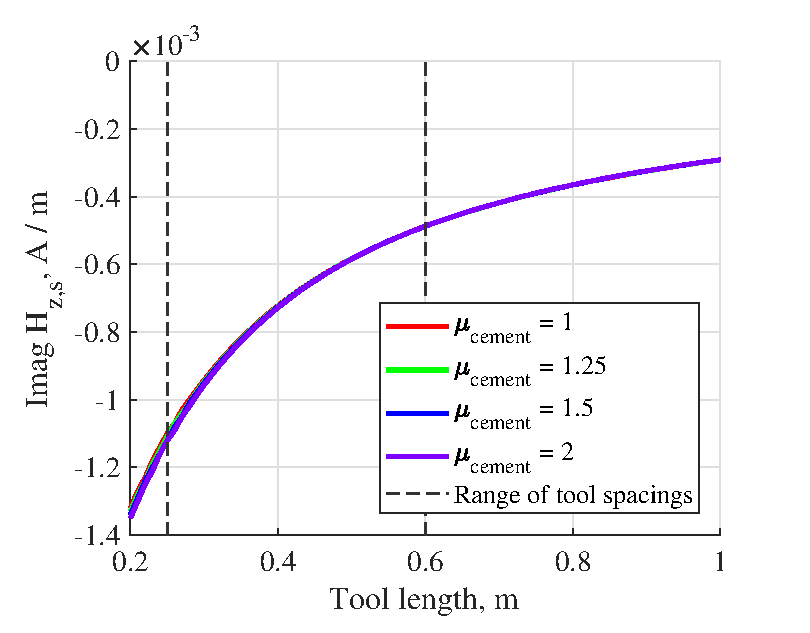
\includegraphics[clip,scale=0.44]{H_im_mu.eps} \\ }
\end{minipage}


\begin{small}
\begin{itemize}
\item \textcolor{green}{$H_{z,s}$} is \textcolor{blue}{strongly} influenced by amount of magnetic powder
\item For magnetic cement \textcolor{blue}{quality} logging it is better to use tools from 0.25 to 0.6 meters
\item Imaginary part of \textcolor{green}{$H_{z,s}$} is weakly influenced by amount of magnetic powder in the cement 
\end{itemize}
\end{small}

%\begin{center}
%\includegraphics[scale=0.55]{mag_cement.eps}
%\end{center}

\end{frame}

%
%------------------------------------------------
%
\begin{frame}

\frametitle{Induction logging signals, frequency = 1 kHz}


\begin{minipage}{0.49\linewidth}
\center{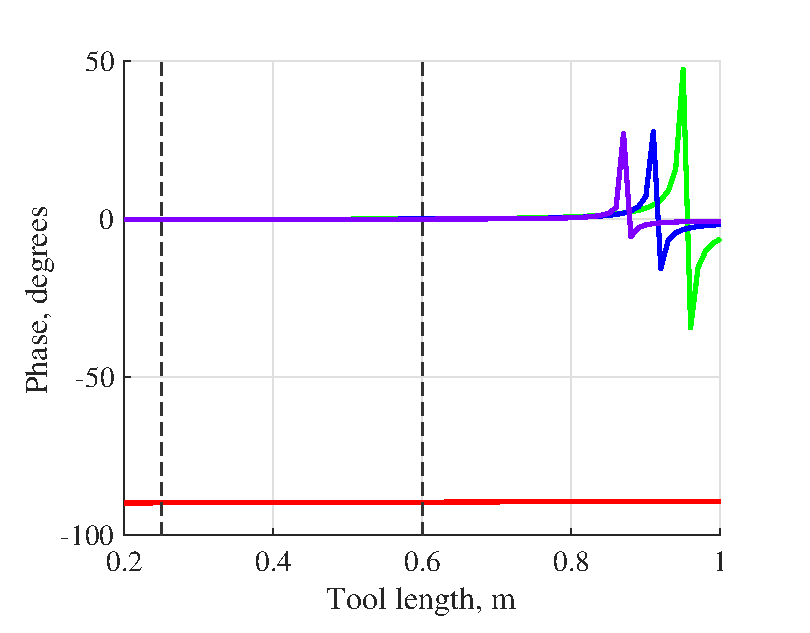
\includegraphics[clip,scale=0.44]{phase_mu.eps} \\ }
\end{minipage}
\hfill
\begin{minipage}{0.49\linewidth}
\center{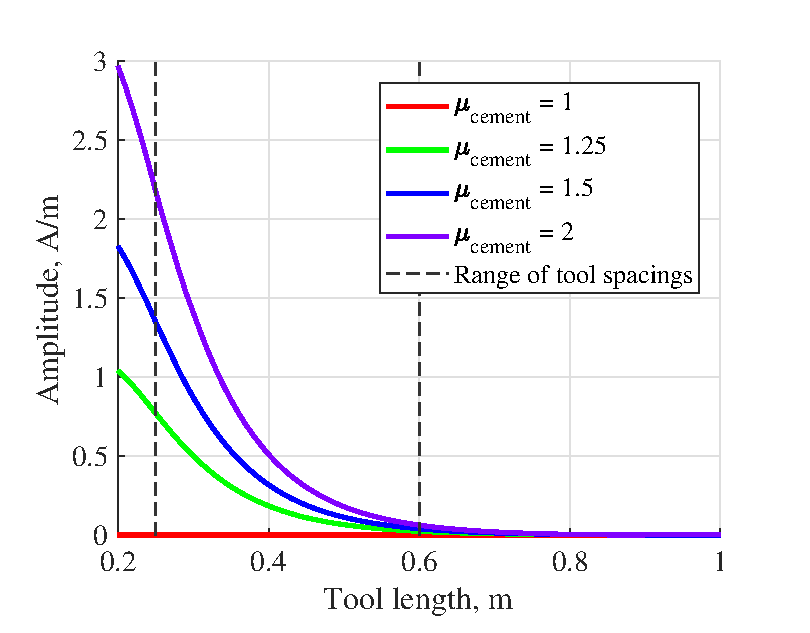
\includegraphics[clip,scale=0.44]{ampl_mu.eps} \\ }
\end{minipage}

\begin{footnotesize}
\begin{equation}
a = Re(H_{z}), b = Im(H_{z}); \hspace{0.5cm} \varphi_m = \arctan \left( \frac{b}{a} \right); \hspace{0.5cm}  A_m =  {\sqrt{a^2+b^2}}
\end{equation}
\end{footnotesize}

$\varphi_m$ - signal phase, $A_m$ - signal amplitude, a and b - real and imaginary parts of $H_z$

%\begin{equation}
%
%
%H_z = k^2 A_z + \frac{\partial^2 A_z}{\partial^2 z}; \;  H_\rho = \frac{\partial^2 A_z}{\partial \rho\partial z}; \; E_\varphi = i \omega \mu \frac{\partial A_z}{\partial \rho}.
%
%
%%a = Re(H_{z}) , \hspace{0.5cm}
%%b = Im(H_{z})
%%%\varphi_m = \arctan \left( \frac{b}{a} \right), \hspace{0.5cm}
%%A_m =  {\sqrt{a^2+b^2}}
%
%\end{equation}
%

%\begin{center}
%\includegraphics[scale=0.55]{mag_cement.eps}
%\end{center}

\end{frame}

%------------------------------------------------
\begin{frame}
\frametitle{Solidification of the cement spotted at frequency = 200 MHz}


\begin{minipage}{0.49\linewidth}
\center{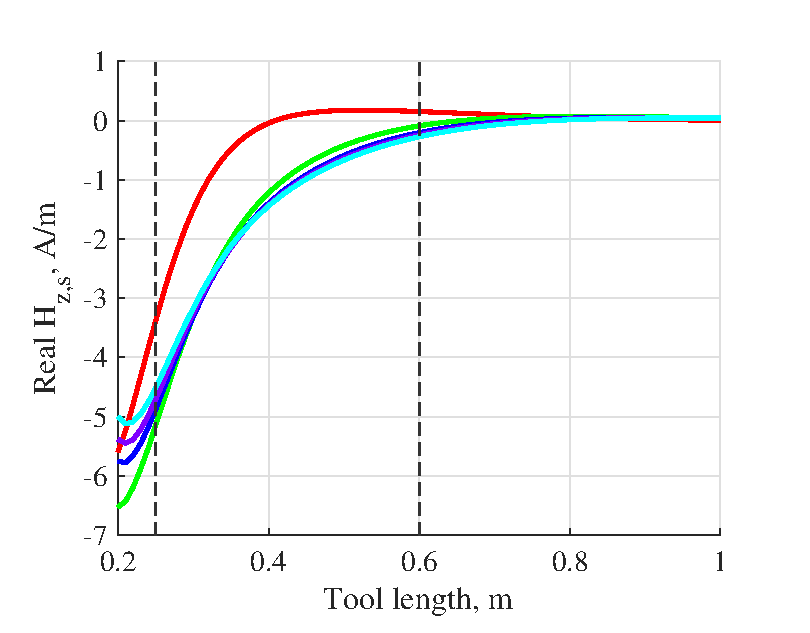
\includegraphics[clip,scale=0.44]{cem_hd_re.eps} \\ }
\end{minipage}
\hfill
\begin{minipage}{0.49\linewidth}
\center{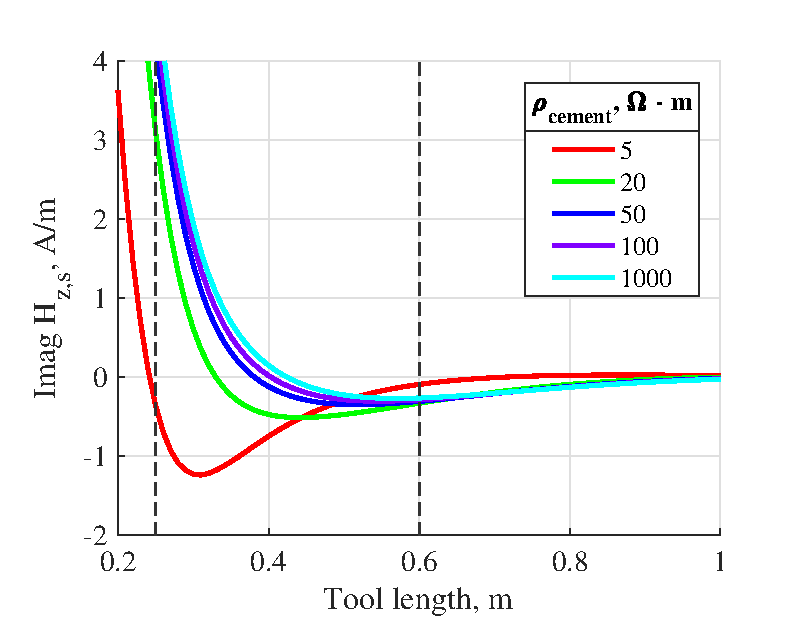
\includegraphics[clip,scale=0.44]{cem_hd_im.eps} \\ }
\end{minipage}


\begin{small}
\begin{itemize}
\item Electrical resistance of cement depends on the degree of its solidification
\item The harder the cement the higher its resistivity
\item Soft cement can be detected at high frequency

\end{itemize}
\end{small}


%Intensity of a) real and b) imaginary part of $H_{z,s}$ vs. tool length at frequency = 200 MHz. Different state of the cement is considered: the harder the cement the higher the resistivity.}

\end{frame}


\begin{frame}
\frametitle{Magnetic cement logging}

Incomplete cement lift and fracture filled with cement can be detected

\begin{minipage}[h]{0.21\linewidth}
\center{\includegraphics[width=1\linewidth]{Borehole_cementlift.eps}} \\
\end{minipage}
\hfill
\begin{minipage}[h]{0.24\linewidth}
\center{\includegraphics[width=1\linewidth]{logging_cemlift.eps}} \\
\end{minipage}
\hfill
\begin{minipage}[h]{0.21\linewidth}
\center{\includegraphics[width=1\linewidth]{Borehole_crack.eps}}  \\
\end{minipage}
\hfill
\begin{minipage}[h]{0.24\linewidth}
\center{\includegraphics[width=1\linewidth]{logging_crack.eps}} \\
\end{minipage}

\end{frame}

%------------------------------------------------

\begin{frame}
\frametitle{Magnetic cement logging}
Cavity filled with cement and 2 cm cement debonding can be detected 

\begin{minipage}[h]{0.21\linewidth}
\center{\includegraphics[width=1\linewidth]{Borehole_cavity.eps}} \\
\end{minipage}
\hfill
\begin{minipage}[h]{0.24\linewidth}
\center{\includegraphics[width=1\linewidth]{logging_cavity.eps}} \\
\end{minipage}
\hfill
\begin{minipage}[h]{0.21\linewidth}
\center{\includegraphics[width=1\linewidth]{Borehole_debonding.eps}} \\
\end{minipage}
\hfill
\begin{minipage}[h]{0.24\linewidth}
\center{\includegraphics[width=1\linewidth]{logging_debond.eps}} \\
\end{minipage}

\end{frame}

%------------------------------------------------

\begin{frame}
\frametitle{Cement hardening logging}


\begin{columns}[c] 

\column{.27\linewidth} 
\begin{small}

A stair-step change of the real and imaginary part can be observed \\
\vspace*{0.2cm}
Magnetic field magnitude changes while logging through different layers \\
\vspace*{0.2cm}
Soft cement can be distinguished from hard one

\end{small}

\column{.18\linewidth} 
\includegraphics[scale=1.4]{cement_solid_model.eps}

\column{.18\linewidth} 
\includegraphics[scale=0.44]{cement_solid_logg_Hre.eps}

\column{.18\linewidth} 
\includegraphics[scale=0.44]{cement_solid_logg_Him.eps}

\end{columns}


\end{frame}


%------------------------------------------------


\begin{frame}
\frametitle{Cement hardening logging, apparent resistivity}


\begin{columns}[c] 

\column{.27\linewidth} 
\begin{small}

Apparent resistivity is calculated from logging signals using homogeneous medium approximation\\
\vspace*{0.2cm}
Resistivity obtained from signal phase is more sensitive to cement resistivity \\
\vspace*{0.2cm}
Singularities can be observed when cross different layers

\end{small}

\column{.18\linewidth} 
\includegraphics[scale=1.4]{cement_solid_model.eps}

\column{.18\linewidth} 

\includegraphics[scale=0.44]{cement_solid_logg_rapp_phs.eps}

\column{.18\linewidth} 

\includegraphics[scale=0.44]{cement_solid_logg_rapp.eps}

\end{columns}


\end{frame}

%------------------------------------------------

\begin{frame}
\frametitle{Eccentricity of the cement}

The eccentricity of cement \textcolor{blue} {can be determined} using a magnetic sensor tool

\begin{columns}[c] 
\column{.45\textwidth} % Right column and width
%{\footnotesize
\includegraphics[scale=1.31]{tool_face_ecctr.eps}

\column{.52\textwidth} % Left column and width

\includegraphics[scale=0.41]{cement_ecctr.eps}
\end{columns}
\end{frame}

%------------------------------------------------

\begin{frame}
\frametitle{Summary}
\begin{itemize}
\item Tools with lengths from 0.25 to 0.6 meters are the most sensitive to the cement properties 
\item Real part of the \textcolor{green}{$H_{z,s}$} for the frequency range from 0.1 kHz to 10 kHz is more sensitive to the magnetic cement
\item Inhomogeneities filled with cement are visible on the logs
\item The absence of cement causes a sharp decrease of magnitude of the secondary magnetic field
\item 200 MHz induction tool can be used for cement solidification detection
\item The proposed method can determine poor-quality cementation through a non-conductive casing
\end{itemize}
\end{frame}
%------------------------------------------------
%\bibliography{TimaRef}
%\bibliographystyle{plainnat}


\end{document} 
